\documentclass[../main.tex]{subfiles}

\begin{document}

\chapter{Literature Review}
\label{chap:lit_review}
In this literature review, we aim to tell you a story of research which has been done in this area of research before this point in time. In doing this we hope to provide the reader of this thesis an understanding of the strengths and weaknesses of relevant literature. What has and what hasn't been done by other researchers. We also will take some time to delve into the papers most relevant to this project by discussing methods and results which we at least considered using in the process of doing our research.\medskip

This literature review will be structured to look at specific topics which are somehow related to the research we carried out. These topics are included in the left hand column of the table below, alongside with the counts for the numbers of papers we looked at for each topic.

If the reader is looking for a good overview of recent climate science it is worth reading \cite{doi:10.1175/2019BAMSStateoftheClimate.1}.


\section{Sea ice trends and variability in Antarctica}
\gls{sie} in Antarctica has changed over the last few years as discussed by \cite{Parkinson2019}. They discuss in detail the behaviour of ice between 1979 and 2018. There has been a steady, although slow increase over the majority of the time period. Despite this steady increase in \gls{sie}, we see a dramatic decrease in \gls{sie} between 2014, where we have our maximum ammount of \gls{sie} of \textcolor{red}{get value} and 2017, where we see the minimum ammount of \gls{sie}. This decrease is larger than any trends seen even in the Arctic, where large decreases in sea ice has been observed. The exact drivers of this are uncertain, although a number of theories have been proposed. This will be discussed in more detail later in this literature review.

Spatial variability is also important for understanding ice in Antarctica fully. Parkinson expands on this by calculating the trends and behaviours seen in different geographic regions of sea ice concentration. It is worth noting that the only region where we see a decreasing trend in Antarctic Sea Ice is in the western Antarctic Peninsula \textcolor{red}{check geography.} \cite{Yuan2018} discusses this as well. Finding that the \gls{rsr} is the only region in Antarctica where we see a statistically significant increase in \gls{sie} over the entire time period. 

It is important to consider the seasonality of the variability we see in Antarctic \gls{sie} as well. \cite{Simpkins} discuss this in some detail. Large-scale climate circulations such as \gls{sam} and \gls{enso} have negilible impact on the longterm trends in \gls{sie}, however they remain significant, at least on a statistical level, on short-term or seasonal variability. 



\subsection*{Sea ice thickness}
It has been much more dificult to measure the thickness of Antarctic Sea ice, and as such we do not have the same breadth of products for this. The best datasets available at the moment are not continuous and only extend as far back as 2002 \textcolor{red}{double check this}. Consequently there is significantly less research which deals with this as a variable, as opposed to \gls{sie} which is no more than an area measure which is easily taken via satilite.


% \section{Atmospheric trends and variability in Antarctica}
% This section of the literature review will discuss the research papers which we looked at regarding the trends and variability of atmospheric conditions around Antarctica.


% \section{Oceanic trends and variability in Antarctica}
% This section of the literature review will discuss the research papers which we looked at regarding the trends and variability of oceanic conditions around Antarctica.

\section{Sea ice and atmospheric processes}
This section of the literature review will discuss in some detail, the research which has been carried out to investigate the relationship between sea ice and atmospheric processes in Antarctica and globally.

Comiso et al look with some detail at the relationship between sea ice in Antarctica and surface temperature \cite{Comiso}. While their dataset ends in 2015, just before the amount of ice in Antarctica experiences a rapid decrease in concentration, their research intent and their methods are still relevant to us as we look at sea ice in Antarctica today. They provide a good commentary on the quality of the satellite measurements from different sensors, before moving into a correlation analysis, looking at the relationship between surface temperature and sea ice in Antarctica. One thing they do is to break the continent into sections and look at how the correlation changes in each region. Likewise they break the temporal scale into seasons while keeping the overall picture. When looking for other environmental influences they found smaller than expected correlations with patterns like the Southern Annular Mode (SAM), however they speculate that ENSO may be a major contributing factor to the patterns in sea ice in Antarctica. On the whole, they found a positive correlation between the SIE in Antarctica and surface temperature in the same region, with an even larger correlation when you introduce a time-lag. 

In 2016 we saw a record low in Antarctic Sea ice extent. Wang et al \cite{Wang2019} discuss some of the physical processes which could be a cause of this extreme event. Their results indicate to them that this was largely due to naturally occurring variability, nonetheless they are unable to discount a possible role of anthropogenic forcing. They link the extreme concentrations of ice to a anomalous atmospheric circulation over the Indian and western Pacific oceans and unusual internal atmosphere-ocean variability. Of interest to us here are the different atmospheric circulation indices they argue has an impact on the patterns of sea ice concentration in Antarctica. The look at the Indian Ocean Dipole (IOD), Madden Julian Oscillation (MJO), ENSO and SAM, as contributors to this event.


\cite{Meehl2016} wrote one of the key papers for our project so we will use it as a starting point. And explore the literature using its references which seem relevant to this topic. The paper focuses on the impacts on the sudden sea ice retreat in 2016 where we saw record low SIE. The first detail of point is that they classify the sections of their SIE time series by when IPO is positive and negative with a 13 year low-pass Lanczos filter. They associate IPO with acceleration or slowdown of global warming, thus relating it to long term trends in sea ice. (Acceleration in positive phase and slowing in negative phase) They say that the acceleration off antarctic sea ice growth was predominantly driven by negative convective heating anomalies in the tropical Pacific.

They also discuss the sudden decrease seen in 2016. They claim this occurred because of a zonal wave number 3 pattern enhancing meridional flow, and negative SAM values towards the end of the year. The DMI index caused positive SST anomalies in the tropical eastern Indian Ocean and the far-western Pacific. This enhanced convection during SON and indicated by record low OLR for the area 90 E - 150 E and an associated precipitation anomaly.

The main takeaway can be drawn from the end of their introduction; First, teleconnections from strong tropical convection in the eastern Indian Ocean produced surface wind anomalies.
They say that a negative phase of IPO and positive phase of SAM associated with strengthened westerlies moved warm subsurface water upwards due to Ekmann suction (On the long term). Third, a negative phase of SAM and transition to a positive IPO produced warm SSTs to complete a warming of the upper 600m of the ocean.
\medskip

\cite{Doddridge2017} discuss in some detail, some of the impact of SAM on the Antarctic SIE seasonal cycle. Their primary finding is that positive SAM anomalies in summer result in cold SST and anomalous ice growth in the following summer, while negative anomalies in SAM can be associated with a reduction in SIE on the following Autumn. The increase in SAM is notably largest in summer and has been linked to the depletion of stratospheric ozone over Antarctica. They note that other papers have found some evidence of the SAM affecting Antarctic SIE in the Indian Ocean during MJJ, but that it is not well explained by SAM. They mention a two time scale response which can be used to explain this relationship. This is explored by \cite{Ferreira} in some detail and may be related to our research. \cite{Doddridge2017} use composites and regression analysis to look at the relationship between SAM and SIE on a seasonal basis finding the results described above. They find the same signal in the raw and detrended datasets.


\cite{Simpkins2012} and \cite{Kohyama2016} discuss with some technical analysis the impact of long term behaviours between Antarctic SIC with ENSO and SAM.



\cite{Clem2020} establish a link between tropical modes of atmospheric climate and surface air temperature (SAT) over the internal Antarctic region. While this isn't directly Sea ice, it is good physical evidence that these relationships exist which supports our hypothesis that SAM impacts the long term variability of Antarctic SIE.

\cite{Turner2020a} Detail some physical reasons for the decrease in Antarctic SIE in 2016.


\section{Sea ice and oceanic processes}
This section of the literature review will discuss in some detail, the research which has been carried out to investigate the relationship between sea ice and oceanic processes in Antarctica and globally.


\section{Land Ice in Antarctica}
In the chapter \ref{chap:data} of this thesis, we discus the usage of GRACE data sourced from NASA to represent the changes in Antarctic land ice over the last couple of decades. Now, we will discuss what the relevant literature has to say regarding the behaviour of Land ice in Antarctica in the context of this dataset. \cite{Velicogna2014RegionalData} run a statistical analysis of the trends in Antarctic and Greenland land ice masses. They identify regions of significant changes in ice mass and accelerations in the change of ice mass over time. They identify that the majority of mass lost in Antarctica is in the Amundsen Sea and Antarctic peninsular regions. With a total loss of 67 $\pm$ 44 Gt/yr of land ice mass. Below Figure \ref{fig:ice_mass_from_paper} from the paper \textcolor{red}{check I can include this.}
\begin{figure}[hbt!]
    \centering
    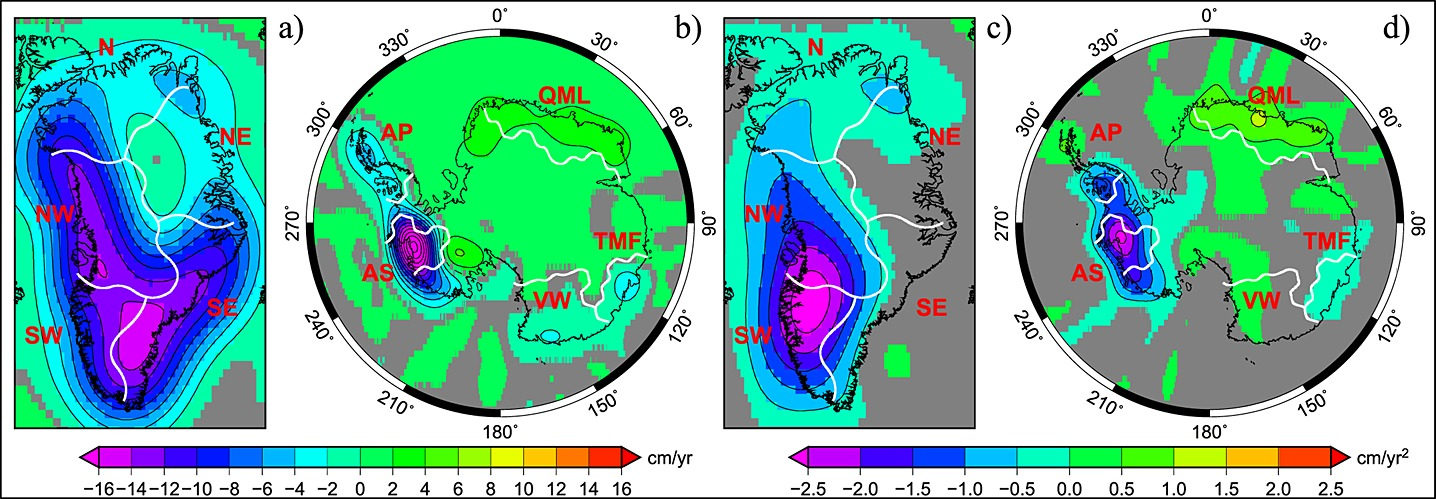
\includegraphics[width=\textwidth]{images/from_papers/grl52143-fig-0001-m.jpg}
    \caption{(a, b) GRACE‐derived Greenland and Antarctica ice mass balance linear trends, dM(t)/dt, in cm/yr of water. (c, d) Accelerations, d2M/dt2, in cm/yr2 for January 2003 to December 2013. Contour interval is 2 cm/yr for the linear trend (Figures a and b) and 0.5 cm/yr2 for the acceleration (Figures c and d). White lines define regions for which time series are calculated in Figure .}
    \label{fig:ice_mass_from_paper}
\end{figure}

This paper links the changes to ice mass with ice dynamics. \cite{Flament2020DynamicAltimetry} discusses this in some detail with examples of glaciers in western Antarctica, the location with the largest amount of ice change. Essentially, glaciers in this region are flowing faster which is causing them to thin. This is linked to warming ocean temperatures which have thinned the ice shelf and ice plain as discussed by \cite{corr_doake_jenkins_vaughan_2001}.

Clouds and the impact they have on the radiative energy balance which in turn has an impact on the Ice-Sheet mass balance could also be another factor to consider. \cite{Scott2017} discuss this in some detail. By looking at a 4-year record of cloud observations and surface radiation measurements they quantify the \gls{wais} radiation budget and investigate the meteorological link between clouds and the trends seen in the ice sheet.

% \section{Statistical Methods}
% This section of the literature review will cover a number of the statistical methods used in different papers which we looked at using for this project. 
% \medskip

% One such technique we may want to use is change-point analysis as discussed by Beaulieu, Chen, and Sarminento \cite{Beaulieu2012}.
% This is used for looking at changes in temporal regimes for time series, they propose it for the purposes of detecting abrupt climate variations. We will also use it for this purpose. The paper provides a good overview of different types of change-points which exist  \textcolor{red}{Include figure?} and a good overview of different ways in which people go about detecting them. They set out to describe and extend an informational approach to this problem, making use of the Schwartz information criterion to identify change points for a variety of fitting models.

\addcontentsline{toc}{chapter}{References}
\bibliographystyle{agsm}
\bibliography{manual_references}


\end{document}